\documentclass[11pt,a4paper]{jarticle}
\usepackage[dvipdfmx]{graphicx}
\usepackage{url}

\renewcommand{\baselinestretch}{1.05} 
\marginparwidth=0cm
\topmargin=-1cm
\headheight=0.3cm
\headsep=0.7cm
\oddsidemargin=0cm
\evensidemargin=0cm
%\textwidth=43zw
\textwidth=15.92cm
%\textheight=43.3\baselineskip
\baselineskip = 0.5744cm
\textheight=43\baselineskip

\itemsep=0.05\baselineskip
\parsep=0pt
\topsep=0.01\baselineskip
\partopsep=0pt
\listparindent=0zw

%% header and footer
\usepackage{fancyhdr}
\pagestyle{fancy}
\lhead{2014年度 春学期授業}
\chead{インタラクティブ・アート実習}
\rhead{担当教員: 松下 光範}
\cfoot{\thepage}
\renewcommand{\headrulewidth}{0pt}
\renewcommand{\footrulewidth}{0pt}

\usepackage{ascmac}
\usepackage{listings,jlisting}
\usepackage{color}
\definecolor{OliveGreen}{cmyk}{0.64,0,0.95,0.40}
\definecolor{colFunc}{rgb}{1,0.07,0.54}
\definecolor{CadetBlue}{cmyk}{0.62,0.57,0.23,0}
\definecolor{Brown}{cmyk}{0,0.81,1,0.60}
\definecolor{colID}{rgb}{0.63,0.44,0}
\definecolor{rulesepcolor}{gray}{0.666}
\lstset{
  language=Java,%プログラミング言語によって変える。
  basicstyle={\ttfamily\small},
  keywordstyle={\color{OliveGreen}},
  %[2][3]はプログラミング言語によってあったり、なかったり
  keywordstyle={[2]\color{colFunc}},
  keywordstyle={[3]\color{CadetBlue}},%
  commentstyle={\color{Brown}},
  %identifierstyle={\color{colID}},
  stringstyle=\color{blue},
  tabsize=2,
  %frame=trBL,
  %numbers=left,
  numberstyle={\ttfamily\small},
  breaklines=true,%折り返し
  %backgroundcolor={\color[gray]{.95}},
  framexleftmargin=0mm,
  frame=single,
  rulesepcolor=\color{rulesepcolor},
  captionpos=b
}


%%%%%%%%%%%%%%%%%%%%%%%%%%%%%%%%%%%%%%%%%%%%%%%%%%%%%%%%%%%%%%%%
\begin{document}

% title
\section*{\LARGE{第3講 スイッチの ON/OFF を取得する}}
Digital Input を用いてスイッチの ON/OFF を取得する。

%%%%%%%%%%%%%%%%%%%%%%%%%%%%%%%%%%%%%%%%%%%%%%%%%%%%%%%%%%%%%%%%

\section{前回の復習}
前回やった Digital Output の復習をしましょう。
ですが、前回やったことをもう一度やるだけではつまらないので、ついでに Processing の新しい命令を覚えましょう。

\subsection*{mousePressed}
mousePressed 変数はマウスが押されているか押されていないかによって、それぞれ true と false に値が変わります。
これを用いると、「マウスがクリックされたときに何かをする」という動作が実現できます。

\begin{lstlisting}
 if (mousePressed) {
   // マウスが押されているときの処理
 } else {
   // マウスが押されていないときの処理
 }
\end{lstlisting}

では、下のプログラムを参考にして前回の内容を思い出しながら、
マウスをクリックしたら LED が点灯する、というプログラムを書いてみましょう。

回路は前回のままで OK です。

\begin{lstlisting}
import processing.serial.*;
import cc.arduino.*;
 
Arduino arduino;
int ledPin = 13;
 
void setup() {
  arduino = new Arduino(this, Arduino.list()[0], 57600);
  arduino.pinMode(ledPin, Arduino.OUTPUT);
}
 
void draw() {
  if (mousePressed) {
    // ここに命令を追加する
  } else {
    // ここに命令を追加する
  }
}
\end{lstlisting}

\subsubsection*{ヒント}
\begin{lstlisting}
 arduino.digitalWrite(n, Arduino.HIGH); // n 番ピンを High (5V) に
 arduino.digitalWrite(n, Arduino.LOW);  // n 番ピンを Low (5V) に
\end{lstlisting}


\section{Digital Input}
ここからが本題です。
Arduino の Digital Input を用いてスイッチの ON/OFF を取得してみましょう。


\subsection*{プルアップ/プルダウン抵抗}
デジタル回路の場合、入力端子がどこにも接続されていないような状態 (オープン) が起こると、電圧が High(5V) または Low(0V) に定まらず誤動作の原因になります。
そのため、マイコンの入力信号がHighかLowかを確実に伝えるために、プルアップ/プルダウン抵抗が必要となります。

%例えスイッチはOFFの状態でも、静電気や電磁誘導によって、電流が生じてしまう。
%マイコンの入力信号がHigh(5V)かLow(0V)かを確実に伝えるために、プルアップ/プルダウン抵抗が必要となります。

\subsubsection{回路を組む}
\begin{figure}[h!]
 \begin{minipage}{0.5\columnwidth}
  \centering
  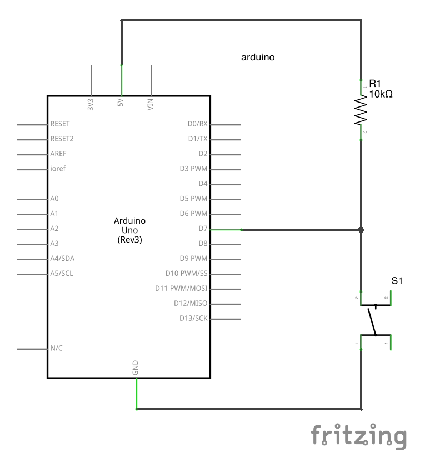
\includegraphics[width=0.7\columnwidth]{img/pullup.eps}
 \end{minipage}
 \begin{minipage}{0.5\columnwidth}
  \centering
  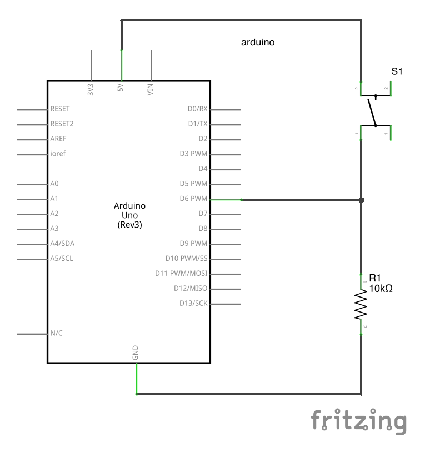
\includegraphics[width=0.7\columnwidth]{img/pulldown.eps}
 \end{minipage}
  \caption{プルアップ抵抗 (左) とプルダウン抵抗 (右)}
\end{figure}

\subsection*{プルアップ抵抗}
\begin{figure}[htbp]
 \begin{minipage}{0.5\columnwidth}
 図\ref{fig:pullupSwitchOff}を見ると、5V側に抵抗が付いています。これをプルアップ抵抗と言います。
 
 スイッチが押されていない時は、図\ref{fig:pullupSwitchOff}の様に抵抗を通してデジタル入力につながるので5Vになり、arduinoではHIGHで読み取られます。
 \end{minipage}
 \begin{minipage}{0.5\columnwidth}
  \centering
  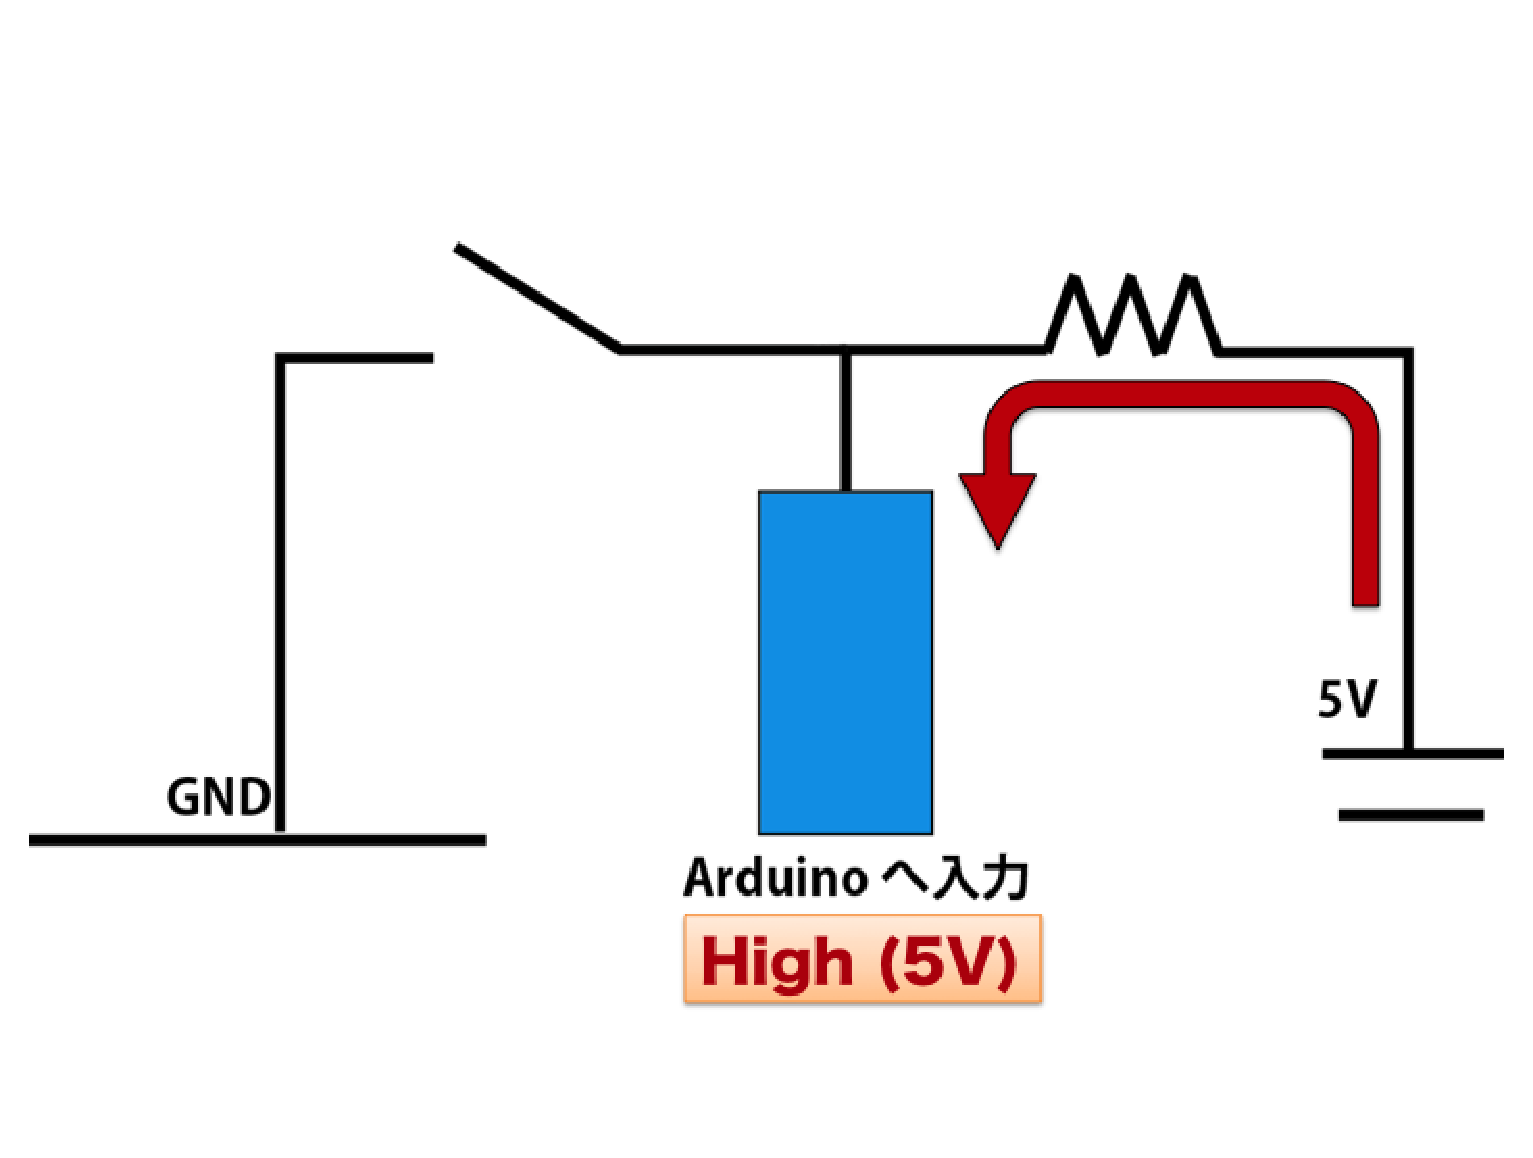
\includegraphics[width=80mm]{img/pullup_off.eps}
  \caption{プルアップ回路 (スイッチが押されていない時) }
  \label{fig:pullupSwitchOff}
 \end{minipage}
\end{figure}

\begin{figure}[htbp]
 \begin{minipage}{0.5\columnwidth}
  スイッチが押された場合は、図\ref{fig:pullupSwitchOn}の様にスイッチを通してGNDとつながるので0Vになります。
  
  電流は青い線のように流れ、デジタル入力側には流れないので0Vになり、arduinoではLOWで読み取られます。
 \end{minipage}
 \begin{minipage}{0.5\columnwidth}
  \centering
  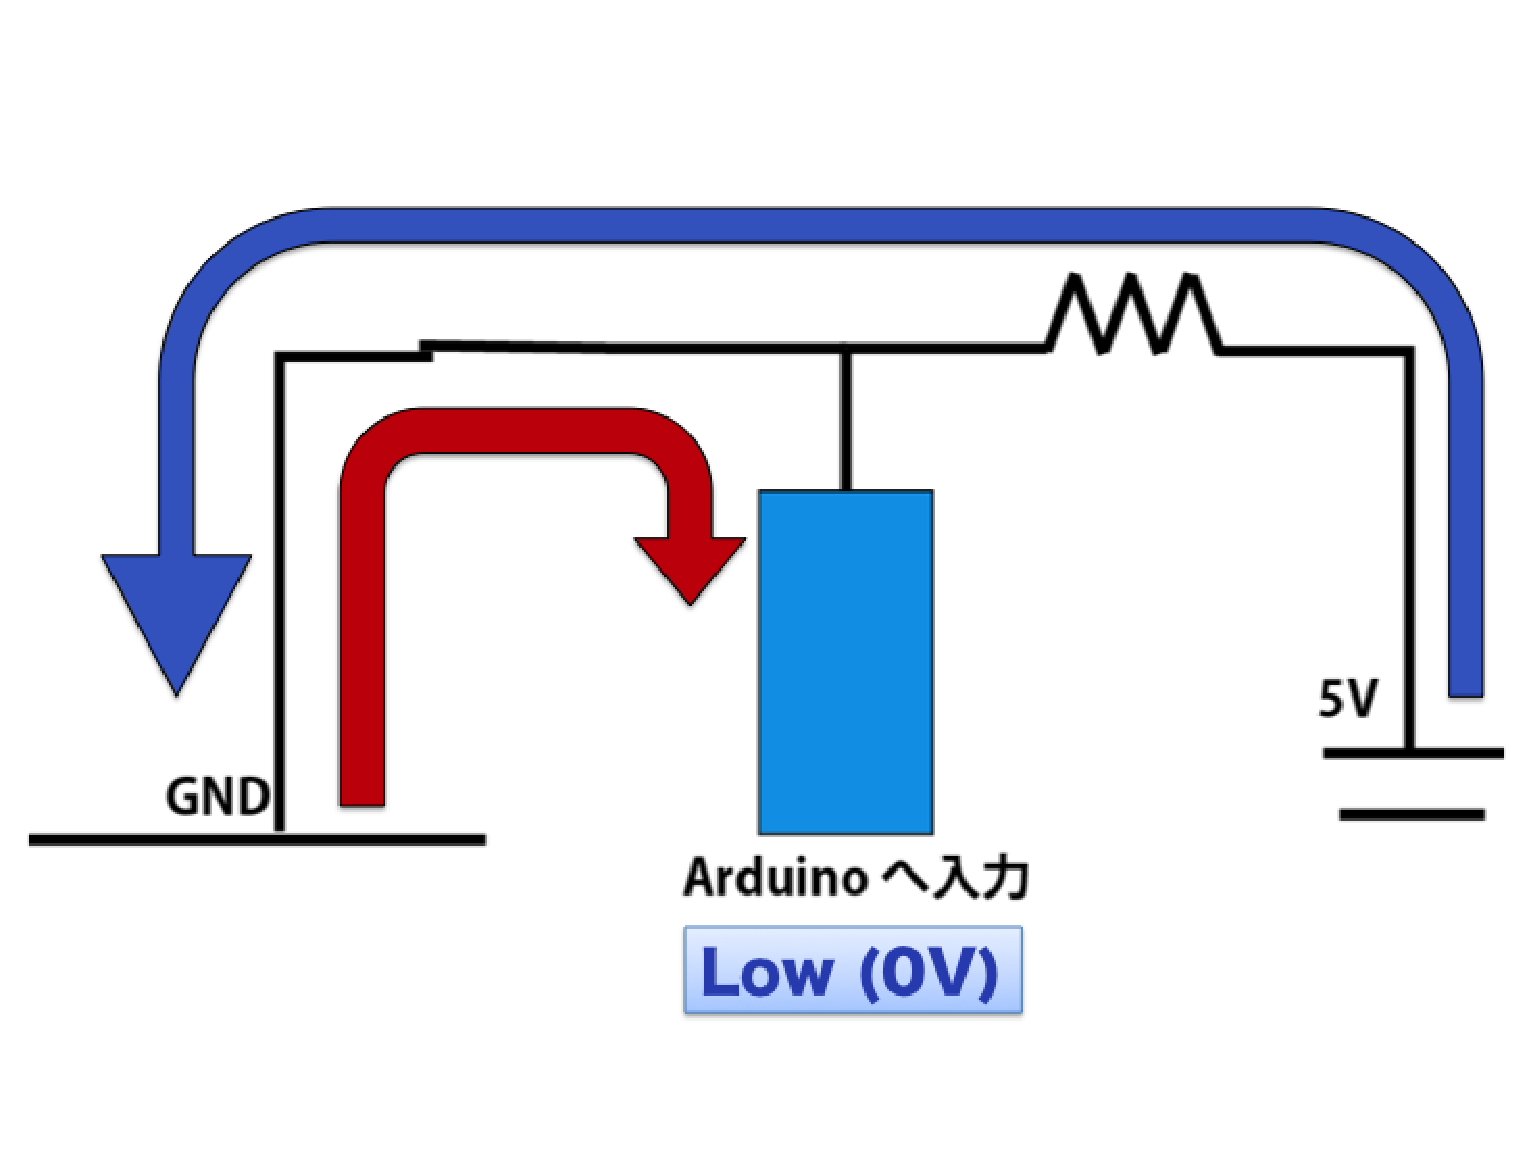
\includegraphics[width=80mm]{img/pullup_on.eps}
  \caption{プルアップ回路 (スイッチが押されている時}
  \label{fig:pullupSwitchOn}
 \end{minipage}
\end{figure}

%\begin{figure}[h!]
% \begin{minipage}{0.5\columnwidth}
%  \centering
% 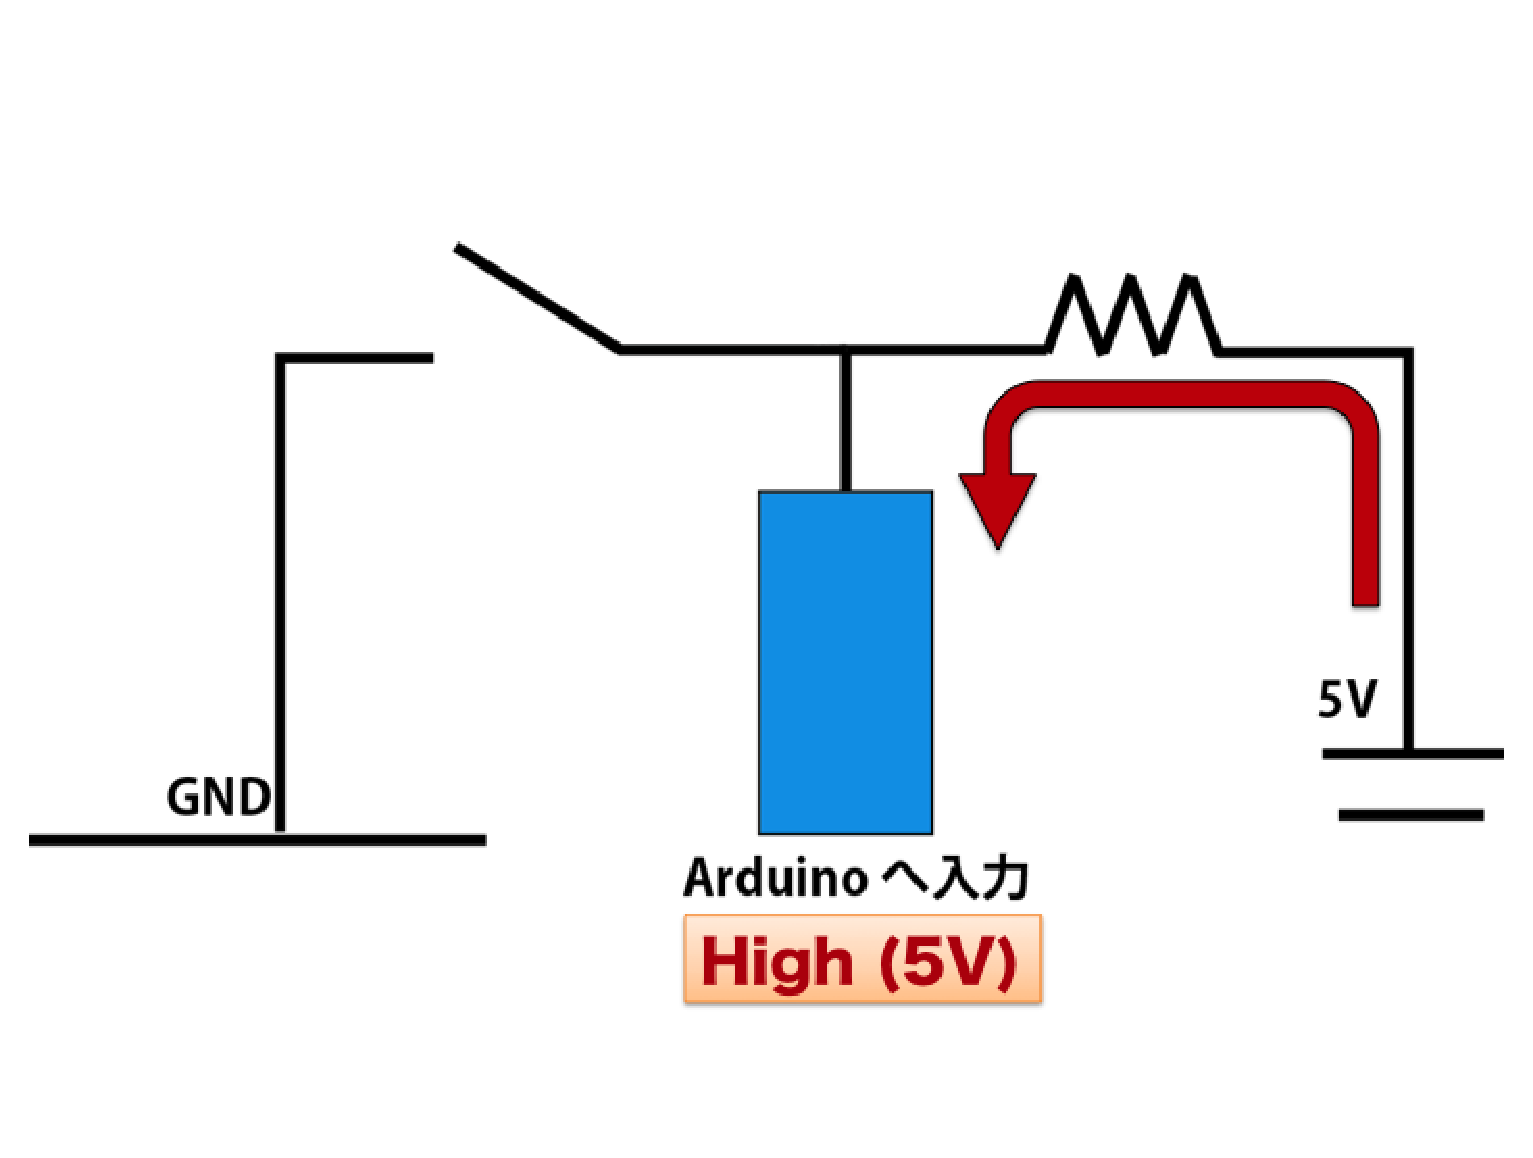
\includegraphics[width=0.9\columnwidth]{img/pullup_off.eps}
% \end{minipage}
% \begin{minipage}{0.5\columnwidth}
%  \centering
%  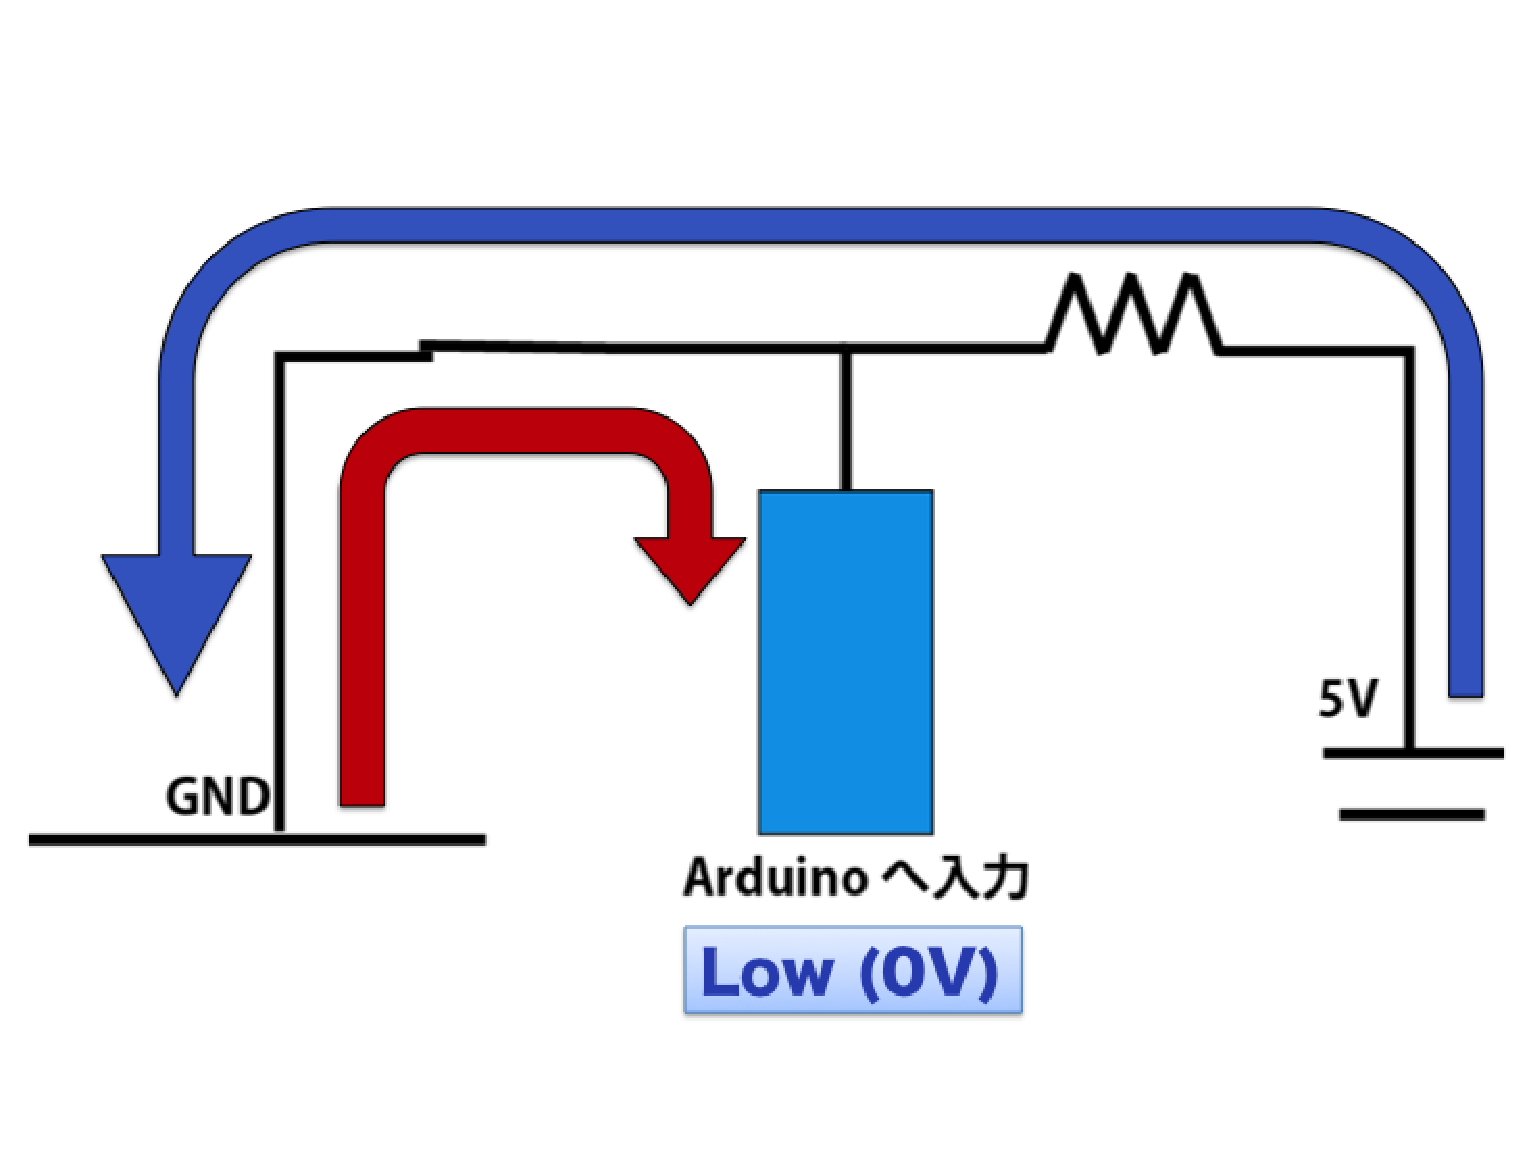
\includegraphics[width=0.9\columnwidth]{img/pullup_on.eps}
%\end{minipage}
%  \caption{プルアップ抵抗ON (左) OFF (右)}
%\end{figure}

 
\subsection*{プルダウン抵抗}
\begin{figure}[h!]
 \begin{minipage}{0.5\columnwidth}
 図\ref{fig:pulldownSwitchOff}を見ると、GND側に抵抗が付いています。これをプルダウン抵抗と言います。
 スイッチが押されていない時は、図\ref{fig:pulldownSwitchOff}のように抵抗を通してデジタル入力はGNDとつながるので0Vになり、arduinoではLOWで読み取られます。
 \end{minipage}
 \begin{minipage}{0.5\columnwidth}
  \centering
  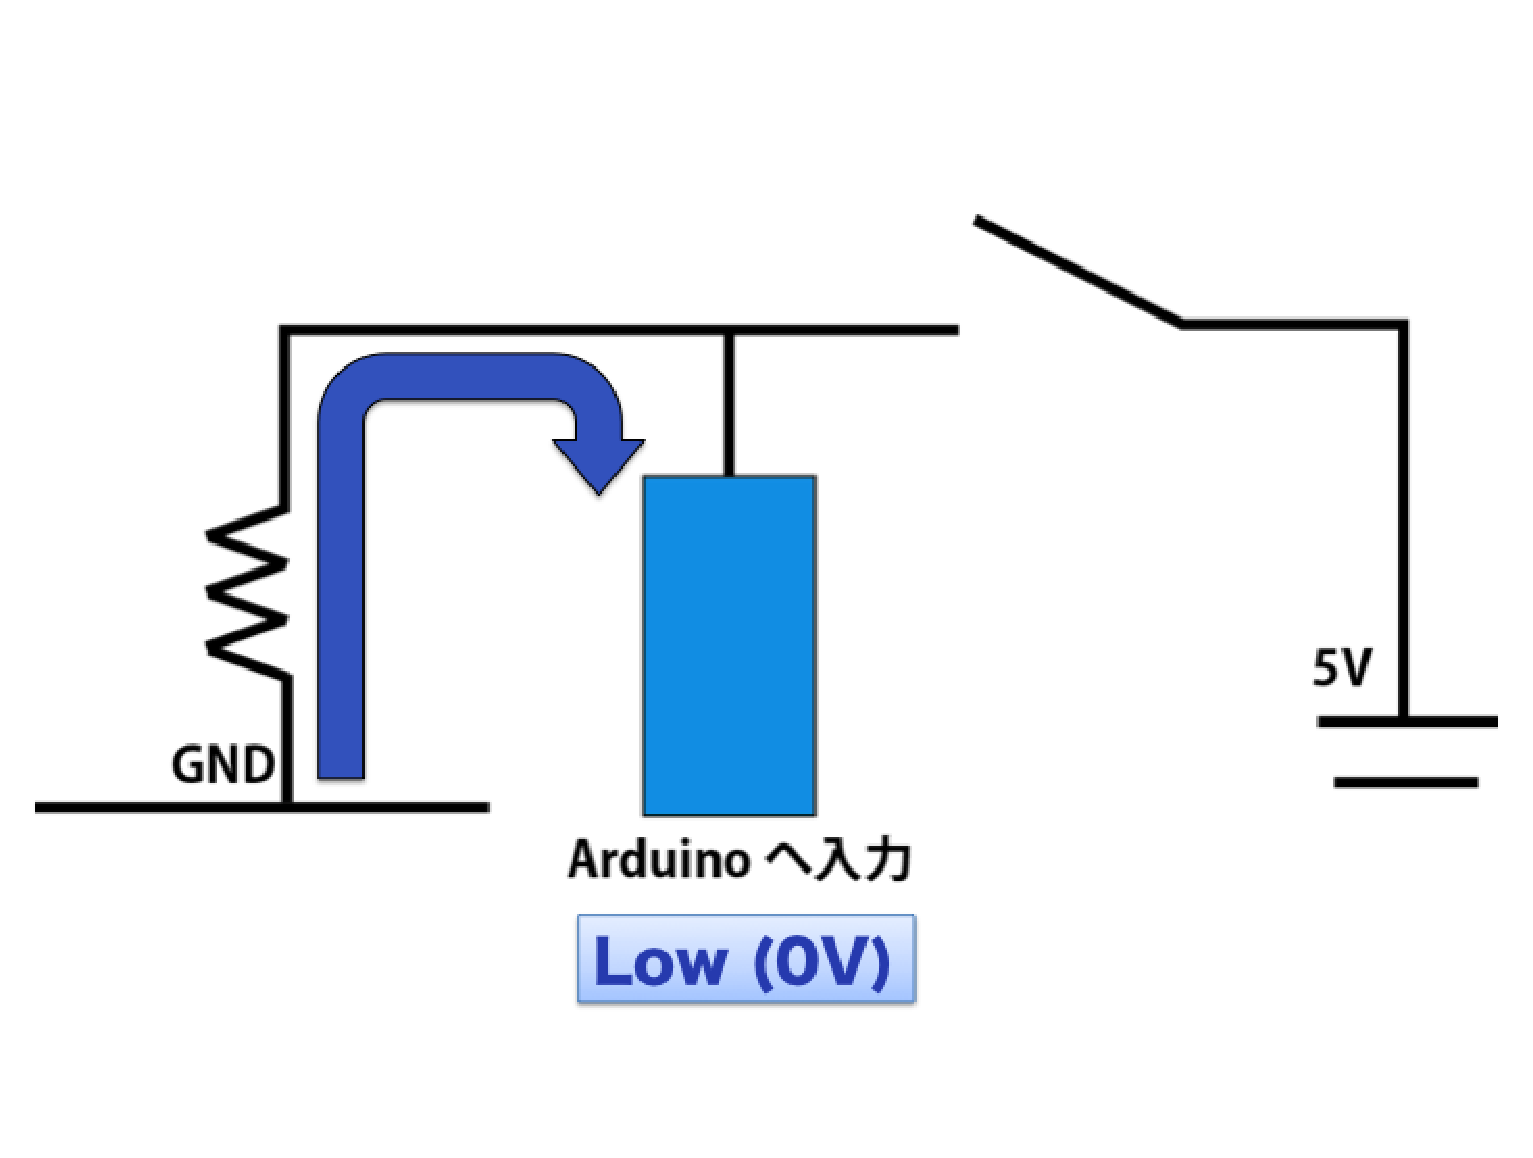
\includegraphics[width=80mm]{img/pulldown_off.eps}
  \caption{プルダウン抵抗OFF状態}
  \label{fig:pulldownSwitchOff}
 \end{minipage}
\end{figure}

\begin{figure}[h!]
 \begin{minipage}{0.5\columnwidth}
  スイッチが押された場合は、図\ref{fig:pulldownSwitchOn}のようにスイッチを通して5Vとつながるのでデジタル入力は5Vになります。
  
  電流は青い線のように流れます。
  
  arduinoではHIGHで読み取られます。
 \end{minipage}
 \begin{minipage}{0.5\columnwidth}
  \centering
  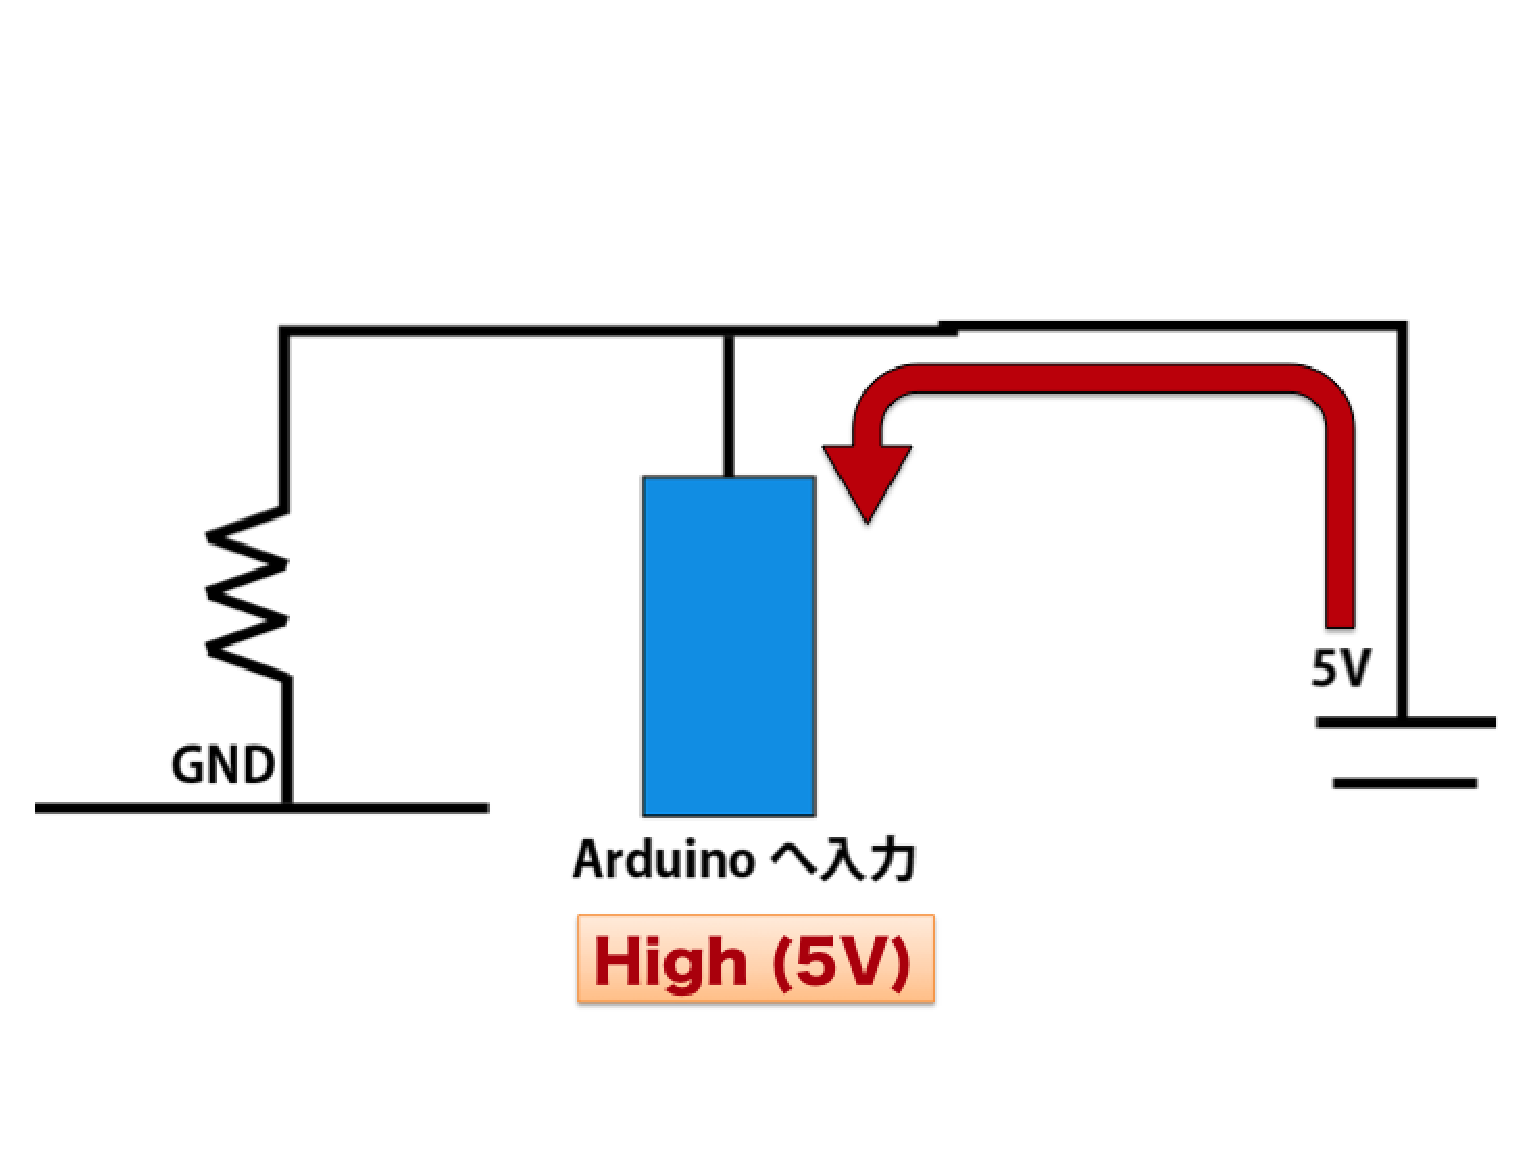
\includegraphics[width=80mm]{img/pulldown_on.eps}
  \caption{プルダウン抵抗ON状態}
  \label{fig:pulldownSwitchOn}
 \end{minipage}
\end{figure}

%\begin{figure}[h!]
% \begin{minipage}{0.5\columnwidth}
  %\centering
 % 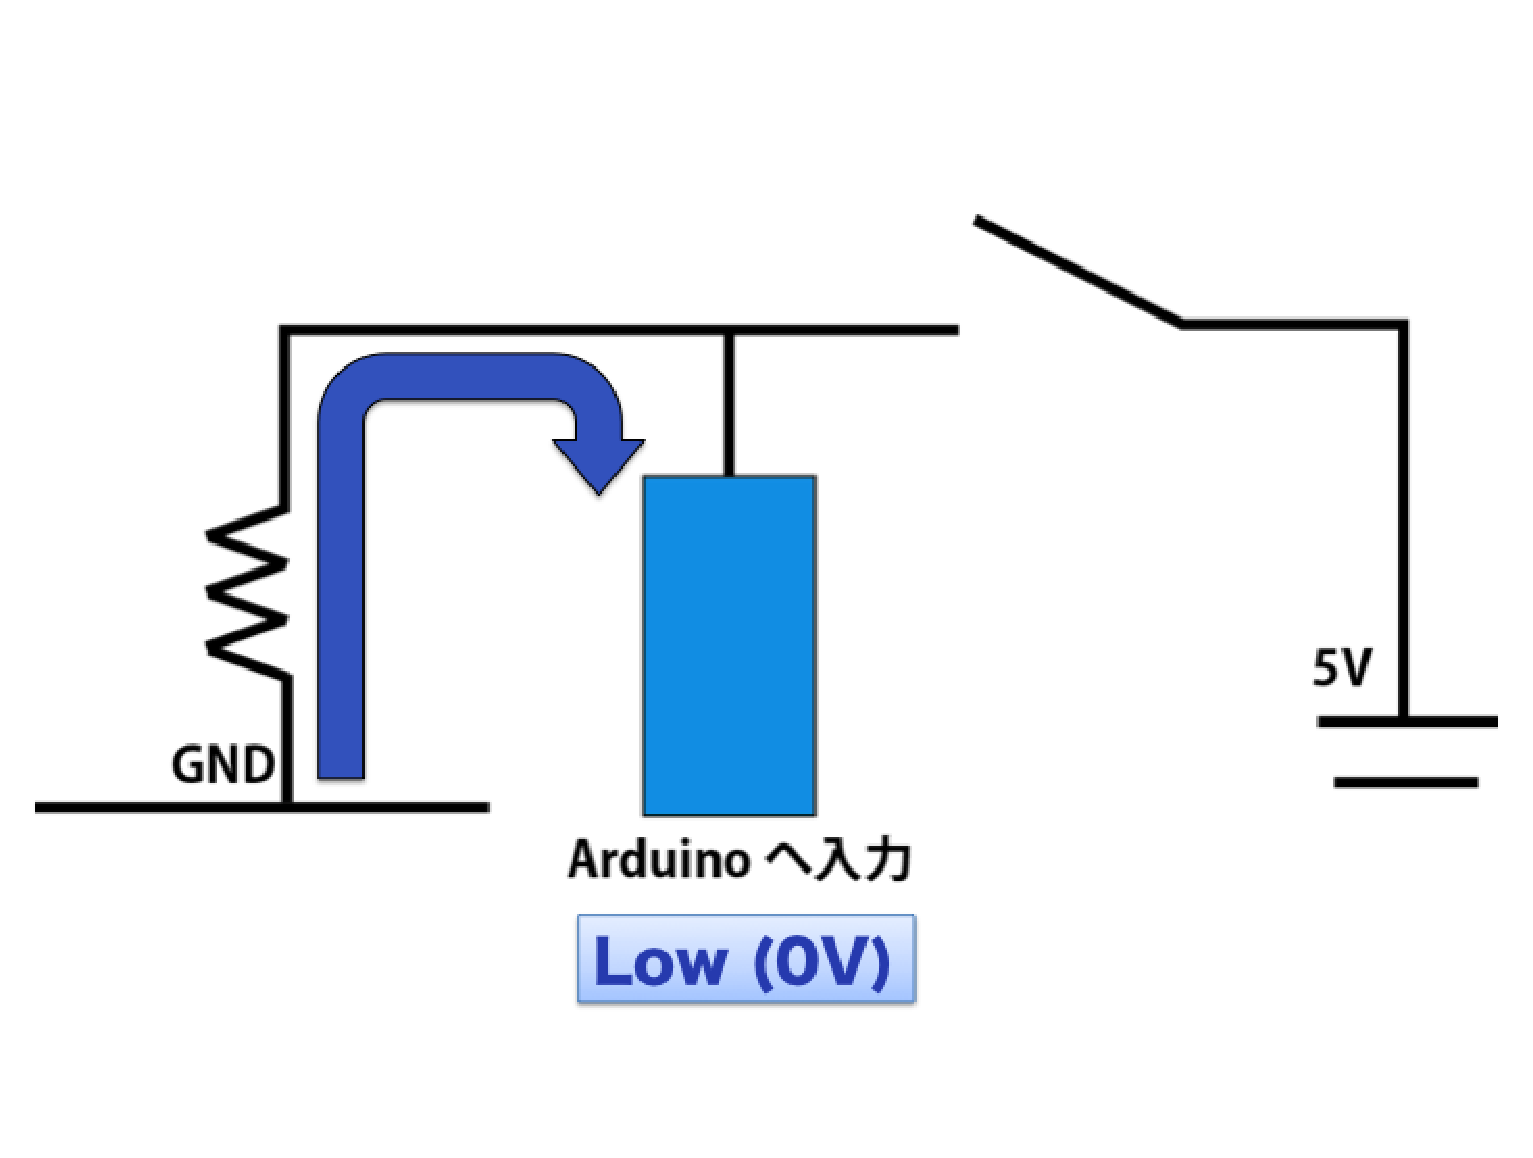
\includegraphics[width=0.9\columnwidth]{img/pulldown_off.eps}
% \end{minipage}
% \begin{minipage}{0.5\columnwidth}
 % \centering
 % 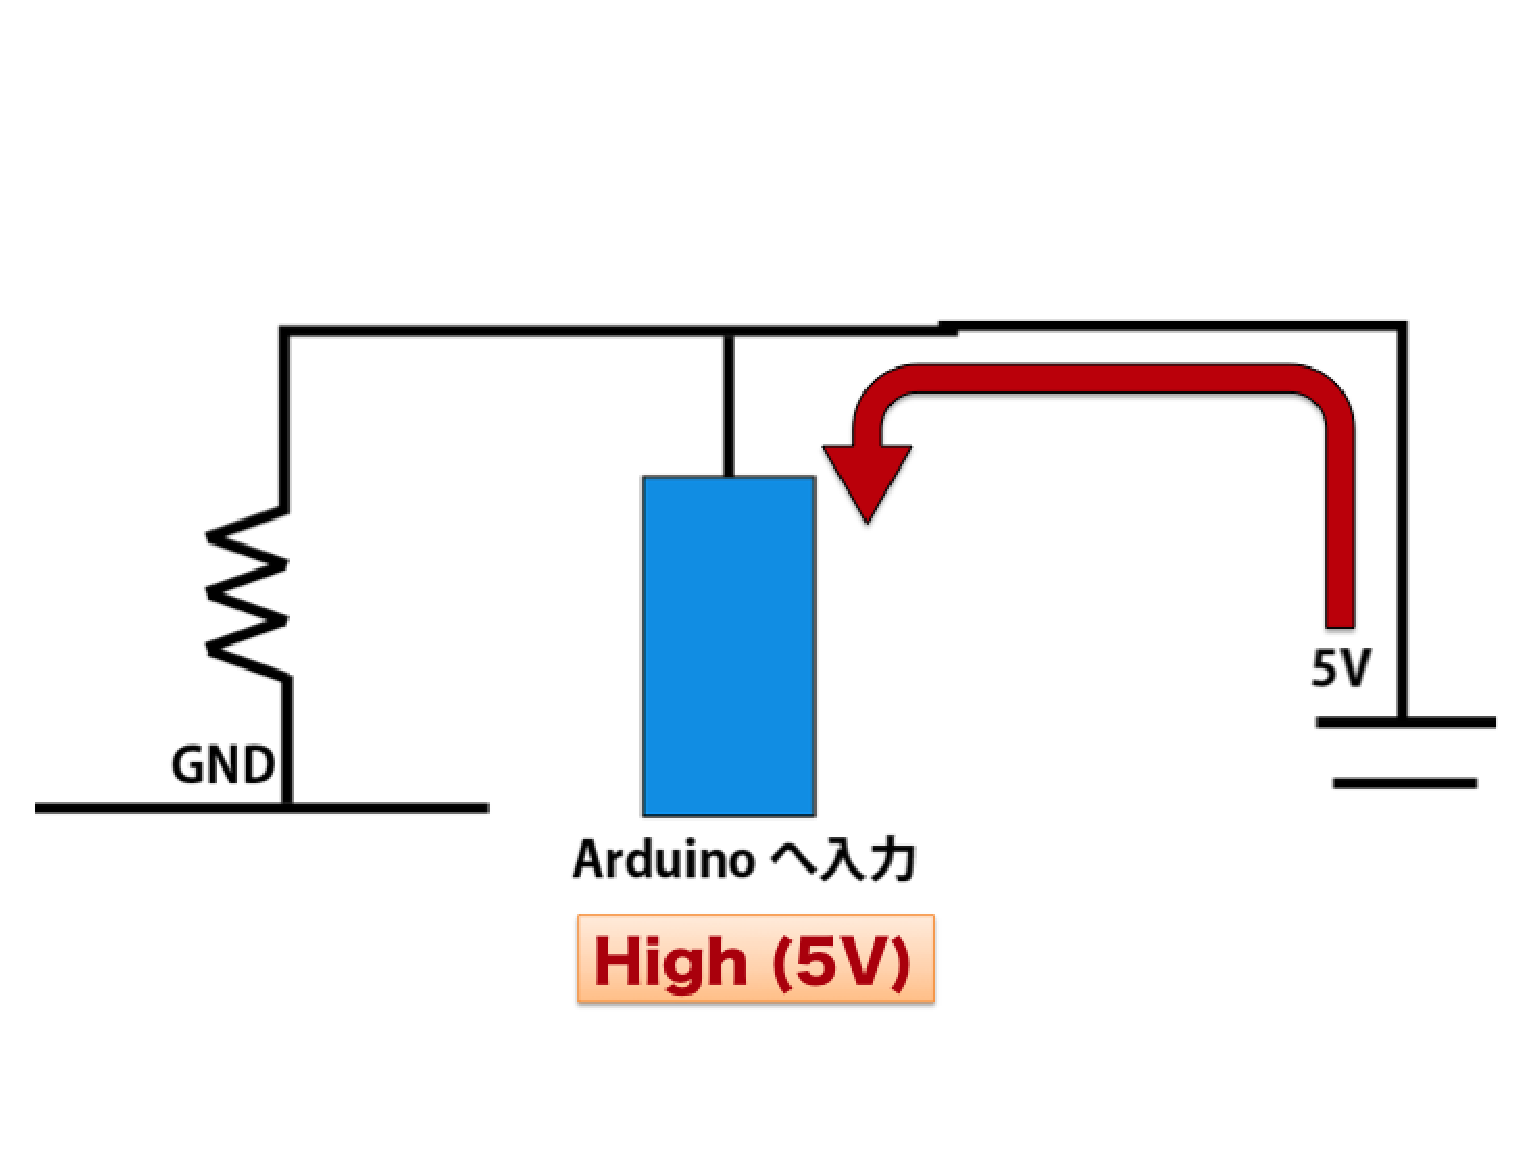
\includegraphics[width=0.9\columnwidth]{img/pulldown_on.eps}
 %\end{minipage}
 % \caption{プルダウン抵抗ON (左) OFF (右)}
%\end{figure}

\subsubsection{プログラムを書く}
\begin{lstlisting}
import processing.serial.*;
import cc.arduino.*;

Arduino arduino;
int switchPin = 8; // スイッチを接続したピンの番号
 
void setup() {
  size(400, 300);
  arduino = new Arduino(this, Arduino.list()[0], 57600);
  arduino.pinMode(switchPin, Arduino.INPUT); // ピンモードを Input に
}
 
void draw() {
  // 8番ピンの電圧を取得し、それが HIGH ならば
  if (arduino.digitalRead(switchPin) == Arduino.HIGH) {
    background(255, 0, 0); // 背景を赤に
  } else {
    background(0, 0, 0);   // そうでなければ (LOW ならば) 背景を黒に
  }
}
\end{lstlisting}

\section{Digital Input と Digital Output を組み合わせる}
スイッチの入力を Processing で取得し、それに基づいて LED を制御しましょう。
前回やった Digital Input と今回やった Digital Output の合わせ技です。

これで入力と出力の両方が実現できるようになります。
次回以降の実習でも入力や出力のための部品が変わるだけで基本的な考え方は同じです。

\subsection*{TRY}
前回と今回やったことを思い出しながら、回路とプログラムを作成してみましょう。
\end{document}

